\documentclass[a4paper,UKenglish]{article}
\usepackage[T1]{fontenc} 

\pdfoutput=1

\usepackage{hyperref}
\bibliographystyle{plain}


\usepackage{graphicx}
\usepackage{epstopdf}

\usepackage{subcaption}

\usepackage{amsmath}
\usepackage{amsfonts}

\usepackage{calc}

\usepackage{caption}

\usepackage{amsthm}
\newtheorem{theorem}{Theorem}
\newtheorem{definition}{Definition}
\newtheorem{lemma}{Lemma}
\newtheorem{corollary}{Corollary}
\newtheorem{remark*}{Remark}
\newtheorem*{openprob*}{Open Problem}
\newtheorem*{conjecture*}{Conjecture}
\newtheorem*{example*}{Example}
\newtheorem*{note*}{Note}
\newtheorem*{prob*}{Problem}
\newtheorem*{acknowledgements*}{Acknowledgements}

\usepackage{tikz}
\usepackage{authblk}

\usepackage[ruled,vlined,nofillcomment,longend,linesnumbered]{algorithm2e}
\newlength\algowd
\def\savewd#1{\setbox0=\hbox{#1\hspace{.7in}}\algowd=\wd0\relax#1}
\newcommand\algolines[2]{\savewd{#1}\tcp*{\parbox[t]{\dimexpr\algowidth-\algowd}{#2}}}



\usepackage{enumitem}





\allowdisplaybreaks
\sloppy



\title{The complexity of optimal design of temporally connected graphs.}

\author[1]{Eleni C. Akrida}
\author[1]{Leszek G\k{a}sieniec}
\author[2]{George B. Mertzios}
\author[1]{Paul G. Spirakis}
\affil[1]{Department of Computer Science, University of Liverpool, UK\\
  \texttt{\{Eleni.Akrida,L.A.Gasieniec,P.Spirakis\}@liverpool.ac.uk}}
\affil[2]{School of Engineering and Computing Sciences, Durham University, UK\\
  \texttt{George.Mertzios@durham.ac.uk}}

\begin{document}

\maketitle

\begin{abstract}
We study the design of small cost temporally connected graphs, under various constraints. We mainly consider undirected graphs of  vertices, where each edge has an associated set of discrete availability instances (labels). A journey from vertex  to vertex  is a path from  to  where successive path edges have strictly increasing labels. A graph is temporally connected iff there is a -journey for any pair of vertices . We first give a simple polynomial-time algorithm to check whether a given temporal graph is temporally connected. We then consider the case in which a designer of temporal graphs can \emph{freely choose} availability instances for all edges and aims for temporal connectivity with very small \emph{cost}; the cost is the total number of availability instances used. We achieve this via a simple polynomial-time procedure which derives designs of cost linear in . We also show that the above procedure is (almost) optimal when the underlying graph is a tree, by proving a lower bound on the cost for any tree. However, there are pragmatic cases where one is not free to design a temporally connected graph anew, but is instead \emph{given} a temporal graph design with the claim that it is temporally connected, and wishes to make it more cost-efficient by removing labels without destroying temporal connectivity (redundant  labels).
Our main technical result is that computing the maximum number of redundant labels is APX-hard, i.e., there is no PTAS unless . On the positive side, we show that in dense graphs with random edge availabilities, there is asymptotically almost surely a very large number of  redundant labels. A temporal design may, however, be \emph{minimal}, i.e., no redundant labels exist. We show the existence of minimal temporal designs with at least  labels.
\end{abstract}

\section{Introduction and motivation}

A temporal network is, roughly speaking, a network that changes with time. A great variety of modern and traditional networks are not static and change over time. For example, social networks, wired or wireless networks may change dynamically, transport network connections may only operate at certain times, etc. Dynamic networks in general have been attracting attention over the past years~\cite{avin,xuan,casteigts,dutta,spirakisc}, exactly because they model real-life applications. In this work, following the model of~\cite{kempe, spirakis} and~\cite{akrida}, we consider \emph{discrete time} and restrict our attention to systems in which only the connections between the participating entities may change but the entities remain unchanged. So we consider networks, the links of which are available only at certain discrete time instances, e.g. days or hours. This is a natural assumption when the dynamicity of the system is inherently discrete, e.g., in synchronous mobile distributed systems that operate in discrete rounds. Moreover, it gives a purely combinatorial flavour to the resulting models and problems.

In several such dynamic settings, maintaining connections may come at a cost; consider the transport network example above or an unstable chemical or physical structure, where energy is required to keep a link available. We define the cost as the total number of discrete time instances at which the network links become available. We focus on design issues of temporal networks that are temporally connected; a temporal network is temporally connected if information can travel over time from any node to any other node following \emph{journeys}, i.e., paths whose successive edges have strictly increasing availability time instances. If one has absolute freedom to design a small cost temporally connected temporal network on an underlying static network, i.e, choose the edge availabilities, then a reasonable design would be to select a rooted spanning tree and choose appropriate availabilities to construct time-respecting paths from the leaves to the root and \emph{then} from the root back to the leaves. However, in more complicated scenarios one may not be free to \emph{choose} edge availabilities arbitrarily but instead \emph{specific} link availabilities might pre-exist for the network; then, one is able to design a temporally connected temporal network using only the pre-existing availabilities or a subset of them. Imagine a hostile network on a complete graph where availability of a link means a break in its security, e.g., when the guards change shifts, and only then are we able to pass a message through the link. So, if we wish to send information through the network, we may only use the times when the shifts change and it is reasonable to try and do so by using as few of these breaks as possible. In such scenarios, we may need to first verify that the pre-existing edge availabilities indeed define a temporally connected temporal network. Then, we may try to reduce the cost of the design by \emph{removing} unnecessary (redundant) edge availabilities if possible, without loosing temporal connectivity. Consider, again, the clique network of  vertices with one time availability per edge; it is clearly temporally connected with cost . However, it is not straightforward if all these edge availabilities are necessary for temporal connectivity. We resolve here the complexity of finding the maximum number of redundant labels in any given temporal graph.

\subsection{The model and definitions}
It is generally accepted to describe a network topology using a graph, the vertices and edges of which represent the communicating entities and the communication opportunities between them respectively. We consider graphs whose edge availabilities are described by sets of positive integers (labels), one set per edge.
\begin{definition}[Temporal Graph]
Let  be a (di)graph. A temporal graph on  is an ordered triple , where  is an \emph{assignment} of labels to the edges (arcs) of .  is called a \emph{labelling} of .
\end{definition}

\begin{definition}[Time edge]
Let  (resp. ) be an edge (resp. arc) of the underlying (di)graph of a temporal graph and consider a label . The ordered triplet  is called \emph{time edge}.
\end{definition}

Note that an undirected edge  is associated with  time edges, namely both  and  for every .

The labels of an edge (arc)  are the \emph{discrete time instances} at which  is available. In many networks and in several applications, the availability of links comes at a cost. For example, in secure networks there is a cost (per discrete time instance) to keep a link secure. We abstract such considerations by the concept of the \emph{cost} of a temporal graph and wish to have temporal graphs of low cost.
\begin{definition}[Cost of a labelling]
Let  be a temporal (di)graph and  be its labelling. The \emph{cost} of  is defined as .
\end{definition}

A basic assumption that we follow here is that when a message or an entity passes through an available link at time , then it can pass through a subsequent link only at some time  and only at a time at which that link is available. 
\begin{definition}[Journey]
A \emph{temporal path} or \emph{journey}  from a vertex  to a vertex  {\emph (-journey)} is a sequence of time edges , ,  , , such that , for each . We call the last time label, , {\emph arrival time} of the journey.
\end{definition}
\begin{definition}[Foremost journey]
A -journey  in a temporal graph is called \emph{foremost journey} if its arrival time is the minimum arrival time of all -journeys' arrival times, under the labels assigned to the underlying graph's edges. We call this arrival time the \emph{temporal distance}, , of  from .
\end{definition}

In this work, we focus on \emph{temporally connected} temporal graphs, i.e., temporal graphs that have the following property:
\begin{definition}[Property TC]
A temporal (di)graph  satisfies the property TC, or equivalently  satisfies TC on , if for any pair of vertices , there is a -journey \emph{and} a -journey in . A temporal (di)graph that satisfies the property TC is called \emph{temporally connected}.
\end{definition}
\begin{example*}
An undirected complete graph, , is temporally connected under any labelling  with  for every . Indeed, there is a -journey and a -journey between any , namely the time edge  and the time edge  respectively, for any .
\end{example*}

\begin{definition}[Minimal temporal graph]
A temporal graph  over a (strongly) connected (di)graph is \emph{minimal} if  has the property TC, and the removal of any label from any , results in a  that \emph{does not} have the property TC.
\end{definition}
\begin{definition}[Removal profit]
Let  be a temporally connected temporal graph. The \emph{removal profit}  is the largest total number of labels that can be removed from  without violating TC on .
\end{definition}
Here, removal of a label  from  refers to the removal of  only from a particular edge and not from all edges that are assigned label , i.e., if  and we remove  from both  and , it counts as two labels removed from .


Notice that if many edges have the same label, we can encounter \emph{trivial cases} of minimal temporal graphs. For example, the complete graph where every edge appears at time, say , is minimal but there are no journeys of length larger than . To avoid cases where minimality is caused merely due to the assignment of the same label(s) to many (or all) edges, we will often consider a special sub-category of (single-labelled) temporal graphs:
\begin{definition}[SLSE temporal graphs]
A Single-label-single-edge (SLSE) temporal graph is a temporal graph, each edge of which has a single label and no two edges have the same label, i.e., each label is assigned to (at most) a single edge. A labelling that gives an SLSE temporal graph is also called \emph{SLSE labelling}.
\end{definition}




\subsection{Previous work and our contribution}\label{sec:full_paper_related}
In recent years, there is a growing interest in distributed computing systems that are inherently dynamic. For example, temporal dynamics of network flow problems were considered in a set of pioneering papers \cite{skutella1, skutella2,woeginger, tardos}. The model we consider here is very closely related to the single-labelled model of the seminal paper of~\cite{kempe} as well as the multi-labelled model of~\cite{spirakis}. In~\cite{kempe}, the authors consider the case of one \emph{real} label per edge and examine how basic graph properties change when we impose the temporal condition; here, we extend that model by considering multiple labels per edge but we restrict our focus to integer labels. In \cite{spirakis}, the model of~\cite{kempe} is also extended to many labels per edge and the authors mainly examine the number of labels needed for a temporal design of a network to guarantee several graph properties with certainty. The latter also defined the cost notion and, amongst other results, gave an algorithm to compute foremost journeys which can be used to decide property TC. However, the time complexity of that algorithm was pseudo-polynomial, as it was dominated by the cube of the maximum label used in the given labelling.

In fact, the problem of testing whether a dynamic graph is temporally connected has been studied before in various settings~\cite{xuan,whitbeck,barjon}. The authors of~\cite{xuan} propose an algorithm for computing foremost journeys in a model of evolving graphs, where nodes and edges are associated with lists of time intervals, representing their existence over time, and each edge has a traversal time. In a similar setting,~\cite{whitbeck} studies temporal reachability graphs, in which a -edge is present at time  if (in the corresponding time-varying graph) there is a -journey leaving  after  and arriving at  after at most some specified time-interval. In~\cite{barjon}, the authors investigate discrete-time evolving graphs, for which they compute the \emph{transitive closure of journeys}, i.e., a static directed graph whose edges represent potential journeys. The algorithm they propose depends on the maximum label used, the number of vertices, and the maximum number of edges that simultaneously exist.

Here, we show that if the designer of a temporal graph can select edge availabilities freely, then an asymptotically optimal linear-cost (in the size of the graph) design that satisfies TC can be easily obtained (cf. Section~\ref{sec:cost_opt_design}). We give a matching lower bound to indicate optimality, in the case where the underlying graph is a tree. However, there are pragmatic cases where one is not free to design a temporal graph anew; instead, one is \emph{given} a set of possible availabilities per edge with the claim that they satisfy TC and the constraint that they may only use them or a subset of them for their design. We also propose a simple algorithm to verify TC in low polynomial time (cf. Section~\ref{sec:foremost}). The \emph{given} design may also be minimal; we partially characterise minimal designs in Section~\ref{sec:minimal}. On the other hand, there may be some labels of the initial design that can be removed without violating TC (and also result in a lower cost). In this case, how many labels can we remove at best? Our main technical result is that this problem is APX-hard, i.e. it has no PTAS unless . On the positive side, we show that in the case of complete graphs and random graphs, if the labels are also assigned at random, there is aymptotically almost surely a very large number of labels that can be removed without violating TC. A preliminary version of this work appeared in the  Workshop on Approximation and Online Algorithms, WAOA 2015~\cite{akrida-waoa}.

Stochastic aspects and/or survivability of network design were also considered in \cite{gupta,lap1, lap2}.


\subsubsection{Further related work}
Below, we provide a short survey of papers with studies on networks labelled by time units or segments, in addition to the ones mentioned above.
	
\noindent \textbf{Labelled Graphs.} Labelled graphs have been widely used both in Computer Science and in Mathematics, e.g.,~\cite{molloy}. 

\noindent \textbf{Continuous Availabilities (Intervals).} Some authors have assumed the availability of an edge for a whole time-interval [] or multiple such time-intervals and not just for discrete moments as we assume here. Examples of such studies are~\cite{xuan, tardos, akrida-algo}.


\noindent \textbf{Dynamic Distributed Networks.} In recent years, there is a growing interest in distributed computing systems that are inherently dynamic~\cite{angluin, avin, casteigts, clementi, dutta, kuhn, spirakisb, spirakisc, o'dell, sch}.

\noindent \textbf{Distance labelling.} A distance labelling of a graph  is an assignment of unique labels to vertices of  so that the distance between any two vertices can be inferred from their labels alone~\cite{gavoille, katz}.

\noindent \textbf{Random labellings.} Random temporal networks have been considered before, e.g., in~\cite{chaintreau,clementi,akrida}. In~\cite{chaintreau}, the authors model opportunistic mobile networks as a type of random temporal networks, where each edge exists at each time-step with a fixed probability, and show a small diameter in general for that type of networks. In ~\cite{clementi}, the authors examine the speed of information dissemination in a type of dynamic graphs, where each edge exists at each time-step with some probability depending on whether it existed in the previous time-step. The \emph{Expected Temporal Diameter} of the model of (random) temporal graphs that we consider here was first examined in \cite{akrida}. 





\section{A low polynomial time algorithm for deciding TC
}\label{sec:foremost}
In this section, we propose a simple polynomial-time algorithm which, given a temporal (di)graph  and a source vertex , computes a \emph{foremost} -journey, for every , if such a journey exists. Curiously enough, the previously known algorithm was pseudo-polynomial~\cite{spirakis}. Our algorithm significantly improves the running time. In fact, we conjecture it is optimal.




\begin{theorem}
Algorithm \ref{alg:foremost} satisfies the following, for every vertex :
\begin{enumerate}[label=(\alph*)]
\item If , then there exists a foremost journey from  to , the arrival time of which is exactly . This journey can be constructed by following the  pointers in reverse order.
\item If , then no -journey exists.
\item The time complexity of Algorithm \ref{alg:foremost} is dominated by the sorting time of the set of time edges (resp. time arcs).
\end{enumerate}
\end{theorem}
\begin{proof}[Proof sketch]
The algorithm actually considers each existing label in the sequence of time labels, from the smallest to the largest one. For each label considered, it computes the foremost journeys from  which arrive at that time\footnote{One can prove this by induction.}. The algorithm examines each time edge (resp. time arc) exactly once.
\end{proof}

\begin{corollary}
The time complexity of Algorithm \ref{alg:foremost} is .
\end{corollary}
\begin{proof}
The time complexity of the algorithm is dominated by the sorting time of . One can sort  by comparison-based sorting resulting in running time .
\end{proof}

\begin{algorithm}[ht]
\caption{Foremost journey algorithm}
\label{alg:foremost}
\SetAlgoLined

\KwIn{A temporal (di)graph  of  vertices, the set of all time edges (arcs) of which is denoted by ; a designated source vertex }
\KwOut{A foremost -journey from  to all , where such a journey exists; if no -journey exists, then the algorithm reports it.}

Sort  in increasing order of labels \tcc*{Note that }
Let  be the sorted array of time edges (resp. time arcs) according to time labels\;
  \tcc*{The set of vertices to which  has a foremost journey}
\;
\For{all }{
		\;
		\;
}
\For{all time edges (resp. time arcs)  in the order given by }{
			\If{ \textbf{and}  \textbf{and}  }{
				\;
				\;
				\;
			}		
}

\end{algorithm}

\begin{conjecture*}
We conjecture that any algorithm that computes journeys out of a vertex  must sort the time edges (resp. time arcs) by their labels, i.e., we conjecture that Algorithm \ref{alg:foremost} is asymptotically optimal with respect to the running time.
\end{conjecture*}

Note that Algorithm \ref{alg:foremost} can even compute foremost -journeys, if they exist, that \emph{start} from a given time . Simply, one ignores the time edges (arcs) with labels smaller than the start time.






\section{Asymptotically cost-optimal design for TC in undirected graphs.}\label{sec:cost_opt_design}
In this section, we study temporal design issues on connected undirected graphs, so that the resulting temporal graphs are temporally connected. In this scenario, the designer has absolute freedom to choose the edge availabilities of the underlying graph.

\begin{lemma}\label{thm:star}
There is an infinite family of graphs  of  vertices, for which the cost of any labelling that satisfies TC is at least .
\end{lemma}
\begin{proof}
Consider the star graph of  vertices, . Let  be the root and  be the leaves. In any labelling on the star graph, which assigns only one label to two (or more) edges , at least one of the vertices  cannot reach the other via a journey. Therefore, any TC satisfying labelling on the star graph must assign at least  labels to all edges of the graph, except possibly on one edge where it assigns a single label. The TC satisfying labelling which assigns labels  to all edges except for one and label  to the remaining edge has, therefore, minimum cost, namely  (cf.~Figure \ref{fig:star}). 

\begin{figure}[!htb]
\centering
\includegraphics[width=0.3\textwidth]{Figures/star}
\caption{Labelling a star graph in an optimal way}
\label{fig:star}
\end{figure}
\end{proof}



In fact, the result of Lemma \ref{thm:star} is optimal for any tree. Theorem~\ref{thm:thmdesign} shows a lower bound for trees and an asymptotically optimal\footnote{Any connected undirected graph needs at least  labels on its edges to be temporally connected, and we show a TC satisfying labelling of  labels.} way of labelling any connected undirected graph to satisfy TC.


\begin{theorem}\label{thm:thmdesign}
\begin{enumerate}[label=(\alph*)]
\item For any tree  of  vertices and for any labelling  that satisfies the property TC on , the cost of  is .
\item Given a connected undirected graph  of  vertices, we can design a labelling  of cost  that satisfies the property TC on .  can be computed in polynomial time.
\end{enumerate}
\end{theorem}

\begin{proof}
\begin{enumerate}[label=(\alph*)]

\item\label{item:tree_lower_bound} We prove the statement by induction on the number of vertices of the tree.
\begin{description}
\item[\textbf{Base Case.}] \noindent It is easy to see that the statement holds for any tree of  vertices.

\item[\textbf{Induction Hypothesis.}] \noindent Assume that at least  labels are \emph{necessary} to satisfy TC on any tree of  vertices, .

\item[\textbf{Inductive Step.}] \noindent We will show that at least  labels are necessary to satisfy TC on any tree of  vertices.

Let  be an arbitrary tree of  vertices and let  be an arbitrary labelling of  that satisfies TC on . Consider a leaf, , of  and its unique neighbour, . Note that  must assign at least one label to the edge  to ``enable'' a journey between them. Now, let  be the sub-labelling of  on . First, we show that, for  to satisfy TC on , it must be that  satisfies TC on .

Assume, to the contrary, that  does not satisfy TC on . Then, there exist two vertices  such that the only journey(s) from  to  in  go through ; let  be a -journey in . It must be:

for some  and  (cf.~Figure~\ref{fig:journey_through_u}).
\begin{figure}[!htb]
\centering
\includegraphics[width=0.6\textwidth]{Figures/journey_through_u}
\caption{A -journey going through .}
\label{fig:journey_through_u}
\end{figure}

But, then the sub-journey of  which ``ignores'' the time-edges  is still a -journey in , which contradicts the fact that all -journeys in  go through . Therefore,  must satisfy TC on . Since  is a tree of  vertices itself, it must be that  (by Induction Hypothesis).

If , then (since  assigns at least one label to the edge ), we have  and the Theorem holds.

It remains to check the case where  and  satisfies TC on .  must assign at least one label to every edge of  to satisfy TC on it. Also, it must assign exactly one label to at least one edge ; if all edges of  had at least two labels under , then it would be . Let  be the unique label of the edge . Also, without loss of generality, assume that  is furthest from  than  is, i.e., the unique path from  to  goes through . For  to enable a -journey in , it must assign to the edge  (at least) one label  that is strictly smaller than . Also, to enable a -journey,  must assign to the edge  (at least) one label  that is strictly greater than  and, thus, different from label  (cf~Figure~\ref{fig:journey_from_u_to_x}). So,  assigns to  at least two labels, which makes the cost of :


\begin{figure}[!htb]
\centering
\includegraphics[width=0.6\textwidth]{Figures/journey_from_u_to_x}
\caption{ must assign to  at least  labels.}
\label{fig:journey_from_u_to_x}
\end{figure}

Therefore, in any case, for  to satisfy TC on , it needs to have cost .
\end{description}









\item\label{item:labelling} Consider a fixed, but arbitrary, spanning tree  of  and let  be the root of . Let  be the length of the longest path from  to any leaf of , i.e.,  is the radius of . We assign labels to the edges of  as follows:
\begin{description}
\item[\textbf{Going upwards.}] Any edge incident to a leaf of  gets label . Any edge , with , where the subtree  rooted at  has been labelled going upwards to the root, gets a label ~(cf.~Figure~\ref{fig:subtree}).
\begin{figure}[!htb]
\centering
\includegraphics[width=0.3\textwidth]{Figures/subtree}
\caption{Labelling ``going upwards'' to the root}
\label{fig:subtree}
\end{figure}
\item[\textbf{Going downwards.}] Any edge incident to the root gets a label . Any edge  in a path from the root to a leaf, the \emph{parent edge}\footnote{The edge before it in the sequence of edges from the root to the respective leaf.} of which has been labelled, going downwards, with label , gets a label .
\end{description}
We can easily implement the above process by topologically ordering the vertices of  in levels using \emph{Breadth First Search} and implement the ``going upwards'' and ``going downwards'' procedures accordingly. The above method results in a labelling where:
\begin{enumerate}[label=\arabic*., ref=\arabic*]
\item each edge of  has  labels,
\item each edge of  has no label and
\item\label{item:c} for each ordered pair of vertices , there is a -journey.
\end{enumerate}
To show \ref{item:c}, just notice that one can go from any vertex  to any other vertex  by going up in  from  to  and then going down in  from  to  via strictly increasing labels, by construction.
\end{enumerate}
\end{proof}

\begin{example*} Figure \ref{fig:example} shows an example of the procedure described above. Notice the existence of journeys from any vertex to every other vertex in the resulting temporal graph.
\begin{figure}[!htb]
\centering
\includegraphics[width=0.7\textwidth]{Figures/example_design}
\caption{Labelling a connected undirected graph to satisfy TC}
\label{fig:example}
\end{figure}
\end{example*}

\begin{conjecture*}
We conjecture that for any connected undirected graph  of  vertices and for any labelling  that satisfies the property TC on , the cost of  is .
\end{conjecture*}


























\section{Minimal Temporal Designs}\label{sec:minimal}
Suppose now that a temporal graph on a (strongly) connected (di)graph  is \emph{given} to a designer with the claim that it satisfies TC. In this scenario, the designer is allowed to only use the given set of edge availabilities, or a subset of them. If the given design is not minimal, they may wish to remove as many labels as possible, thus reducing the cost. Minimality of a design can be verified by running Algorithm \ref{alg:foremost} (cf.~Section \ref{sec:foremost}) for every .



\subsection{A partial characterisation of minimal temporal graphs}\label{sec:full_paper_hyper}
As mentioned earlier, if many edges have the same label, we can encounter \emph{trivial cases} of minimal temporal graphs. To avoid such cases, we focus our attention here to the class of SLSE temporal graphs, in which every edge only becomes available at one moment in time and no two different edges become available at the same time. Are there minimal SLSE temporal graphs with non linear (in the size of the graph) cost? For example, any complete SLSE temporal graph satisfies TC. Are all these  labels needed for TC, i.e., are there minimal temporal complete graphs? As we prove in Theorem \ref{thm:clique_code}, the answer is negative. However, we give below a minimal temporal graph on  vertices with non-linear in  cost, namely with  labels.


\subsubsection{A minimal temporal design of \texorpdfstring{}{nlogn} cost}\label{sec:nlogn_minimal}

\begin{definition}[Hypercube graph]
The -hypercube graph, commonly denoted , is a -regular graph of  vertices and  edges. The -hypercube is the graph of two vertices and one edge. Recursively, the -hypercube is produced by taking two isomorphic copies of the -hypercube and adding edges between the corresponding vertices.
\end{definition}

\begin{definition}[Flat]
In geometry, a \emph{flat} is a subset of the -dimensional space that is congruent to a Euclidean space of lower dimension, e.g., the flats in the two-dimensional space are points and lines. In the -dimensional space, there are flats of every dimension from , i.e., points, to , i.e., hyperplanes.
\end{definition}
\begin{theorem}
There exists an infinite class of minimal temporal graphs on  vertices with  edges and  labels, such that different edges have different labels.
\end{theorem} 
\begin{proof}
We present a minimal temporal graph on the hypercube graph of  vertices. Consider Protocol \ref{label_protocol'} for labelling the edges of . The temporal graph, , that this labelling procedure produces on the hypercube is minimal. Indeed, first we will prove that the temporal graph produced by Protocol \ref{label_protocol'} satisfies TC on .

Consider vertices  and the steps described in Protocol \ref{journeyQn} to reach , starting from , via temporal edges. The procedure described in Protocol \ref{journeyQn} gives a journey from  to , which is also \emph{unique}. It suffices to consider the -bit binary representation of the vertices of . Notice that if the hamming distance of the labels of two vertices  is exactly , then to reach  from  via a temporal path in the temporal graph on , we need to move through vertices by consecutively swapping the bits in which  and  differ in the order of dimensions. This way, we maintain the strictly increasing order of the time labels we use and, swap by swap, we approach the destination. Note also that swapping only the bits in which  and  differ is the only way to not violate the increasing order of time labels we use: without loss of generality, suppose that the  bit of  is  and so is  bit of . If, starting from , we swap the  bit to , i.e., we use an edge, , on the  dimension, then at a future step, we again need to swap the  bit back to  (otherwise, we never reach ). However, the two swaps cannot be consecutive, because then we would use edge  twice and we violate the increasing order of labels. So, we would need to move to a higher dimension after the first of the two swaps; but, then, we have used labels that are larger than all the labels of the  dimension, so using any edge of the  dimension would also violate the increasing order of labels.
\begin{algorithm}[ht]
\SetAlgorithmName{Protocol}{protocol}{List of protocols}
\caption{Labelling the hypercube graph, }
\label{label_protocol'}
\SetAlgoLined

	Consider the  dimensions of the hypercube , \;
	\For{}{
			Let  be the list of edges in dimension , in an arbitrary order\;
			Let  be the (sorted from smallest to largest) list of labels  \;
	}	
	\For{}{
		\For{}{
				Assign the (current) first label of  to the (current) first edge of  \;
				Remove the (current) first label of  from the list\;
				Remove the (current) first edge of  from the list\;
		}
	}
	\Return{the produced temporal graph, ;}
\end{algorithm}

\begin{algorithm}[ht]
\SetAlgorithmName{Protocol}{protocol}{List of protocols}
\caption{A temporal path from  to  in the temporal graph on }
\label{journeyQn}
\SetAlgoLined

	\KwIn{The considered temporal graph on the hypercube , vertices }
	\KwOut{Array  of vertices, which the -journey passes through}
	\;
	Find the flat of the smallest dimension, , which both  and  lie on\;
	Consider the increasing order of the  dimensions in that flat: \;
	\For{}{
			Use the incident edge of  that lies on dimension  and let  be the other endpoint of that edge\;
	}
\end{algorithm}


Since our labelling gives a \emph{unique} -journey, for every , and since all labels assigned to the edges of  are used in the union of all those journeys, the deletion of any single label will violate TC. Therefore,  is minimal. Finally, note that the temporal graph  on the hypercube graph  has  vertices,  edges and  labels.
\end{proof}

















\subsubsection{A minimal temporal design of linear in \texorpdfstring{}{n} cost}
In the previous section, we showed that there are graphs of non-linear cost (in the number of vertices) that are minimal. Here, we show that there are classes of minimal graphs whose cost is linear in the number of their vertices.


Indeed, as seen in Lemma~\ref{thm:star} (Section~\ref{sec:cost_opt_design}), the star graph of  vertices needs at least  labels to satisfy TC and, in fact, we present there a TC satisfying labelling of  labels (cf.~Figure~\ref{fig:star}). Theorem~\ref{thm:thmdesign}\ref{item:labelling} (Section~\ref{sec:cost_opt_design}) also gives a class of minimal temporal graphs of linear cost in the number of vertices. Therefore, we have the following Corollary:

\begin{corollary}
There exists an infinite class of minimal temporal graphs on  vertices with  edges and  labels.
\end{corollary}








\subsubsection{SLSE Cliques of at least 4 vertices are not minimal}\label{sec:clique_minimal}

The complete graph on  vertices, , with an SLSE labelling , i.e., a labelling that assigns a single label per edge, different labels to different edges, is an interesting case, since  always satisfies TC. However, it is not minimal as the theorem below shows.

\begin{theorem}\label{thm:clique_code}
Let  and denote by  the complete graph on  vertices. There exists \emph{no minimal} SLSE temporal graph on . In fact, we can remove (at least)  labels from any SLSE labelling on  without violating TC.
\end{theorem}
\begin{proof}
The proof is divided in two parts, as follows:
\begin{enumerate}[label=(\alph*)]

\item\label{item:code_a} We first show that any SLSE labelling on the complete graph on  vertices produces a temporal graph that is not minimal, i.e., the theorem holds for . Consider the six different labels  assigned by an SLSE labelling to the edges of  as shown in Figure~\ref{fig:K_4}.

\begin{figure}[tbh!]
\centering
\includegraphics[scale=0.7]{Figures/K_4}
\caption{Any SLSE labelling on  is not minimal.}
\label{fig:K_4}
\end{figure}

Up to their renaming, there are three possible cases for the labels . Counting all the cases of \emph{alternation}, \emph{cycle}, and \emph{entanglement} (see below) would give us all possible  cases.

\begin{enumerate}[label=\arabic*.]
\item (Alternation) .\\It is easy to see that in this case, both diagonals can be removed:  can reach  using labels  and then ;  can reach  using labels  and then ;  can reach  using labels  and then ;  can reach  using labels  and then .
\item (Cycle) .\\Here, diagonal  can be removed:  can reach  using labels  and then ;  can reach  using labels  and then .
\item (Entanglement) .\\This is a more complex case, for which we distinguish the following five sub-cases:
	\begin{enumerate}[label=\roman*)]
	\item  and .\\We can remove label :  can reach  using labels  and then ;  can reach  using labels  and then .
	\item  and .\\We can remove label :  can reach  using labels , then  and then ;  can reach  using labels , then  and then  (notice that ).
	\item  and .\\We can remove label :  can reach  using labels  and then ;  can reach  using labels  and then .
	\item  and .\\We can remove label :  can reach  using labels  and then ;  can reach  using labels , then  and then .
	\item  and .\\We can remove label :  can reach  using labels , then  and then ;  can reach  using labels , then  and then .
	\end{enumerate}
	Notice that the coverage of the above five cases is complete (cf.~Figure~\ref{fig:coverage}).
	\begin{figure}[tbh!]
	\centering

	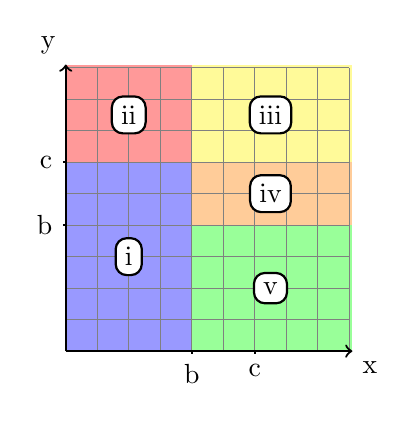
\begin{tikzpicture}[scale=0.4]
	
	\fill[blue!40!white] (0,0) rectangle (4,6);	
	\fill[red!40!white] (0,6) rectangle (4,9.1);
	\fill[yellow!40!white] (4,6) rectangle (9.1,9.1);
	\fill[orange!40!white] (4,4) rectangle (9.1,6);
	\fill[green!40!white] (4,0) rectangle (9.1,4);



	\draw[step=1cm,gray,very thin] (0,0) grid (9,9);
	\draw[thick,->] (0,0) -- (9.1,0) node[anchor=north west] {x};
	\draw[thick,->] (0,0) -- (0,9.1) node[anchor=south east] {y};
	
	\node[rectangle, rounded corners, draw, thick, fill=white] (i) at (2,3) {i};
	\node[rectangle, rounded corners, draw, thick, fill=white] (iii) at (2,7.5) {ii};
	\node[rectangle, rounded corners, draw, thick, fill=white] (ii) at (6.5,7.5) {iii};
	\node[rectangle, rounded corners, draw, thick, fill=white] (v) at (6.5,5) {iv};
	\node[rectangle, rounded corners, draw, thick, fill=white] (iv) at (6.5,2) {v};


	\draw[thick] (4,0) -- (4,-0.1) node[anchor=north] {b};
	\draw[thick] (6,0) -- (6,-0.1) node[anchor=north] {c};
	\draw[thick] (0,4) -- (-0.1,4) node[anchor=east] {b};
	\draw[thick] (0,6) -- (-0.1,6) node[anchor=east] {c};
	
	\end{tikzpicture}

	\caption{The six sub-cases cover all possible scenarios of ``entanglement''.}
	\label{fig:coverage}
	\end{figure}
\end{enumerate}




\item Now, consider the complete graph on  vertices, . Partition  arbitrarily into  subsets , such that  and . In each -clique defined by , we can remove a ``redundant'' label, as shown in~\ref{item:code_a}. The resulting temporal graph on  still preserves TC since for every ordered pair of vertices :
\begin{itemize}
\item if  are in the same , , then there is a -journey that uses time edges within the 4-clique on , as proven in \eqref{item:code_a}.
\item if  and , then there is a -journey that uses the (direct) time edge on .
\end{itemize}
\end{enumerate}
\end{proof}





\subsection{Computing the removal profit is APX-hard}


Note that it is straightforward to check in polynomial time whether a given  satisfies TC on a given (di)graph , by just checking for every possible
(ordered) pair  of vertices in  whether there is a -journey in . Recall that the removal profit is the largest number of labels that can be removed from a temporally connected graph without destroying TC. We now show that it is hard to approximate the value of the removal profit arbitrarily well for an arbitrary
graph, i.e.,~there exists no PTAS\footnote{PTAS stands for Polynomial-Time Approximation Scheme.} for this problem, unless P=NP. It is worth noting here that, in our hardness proof below, we consider \emph{undirected} graphs; the fact that all -journeys,  exist in any given (unlabelled) connected undirected graph makes the reduction and the analysis much more involved.

We prove our hardness result by providing an approximation preserving
polynomial reduction from a variant of the maximum satisfiability problem,
namely from the \emph{monotone Max-XOR()} problem. Consider a monotone
XOR-boolean formula  with variables ,
i.e.,~a boolean formula that is the conjunction of XOR-clauses of the form , where no variable is negated. The clause  is XOR-satisfied by a truth assignment  if and
only if  in . The number of clauses of  that
are XOR-satisfied in  is denoted by . If every
variable  appears in exactly  XOR-clauses in , then 
is called a \emph{monotone XOR(}\emph{)} formula. The \emph{monotone
Max-XOR(}\emph{)} problem is, given a monotone XOR() formula ,
to compute a truth assignment  of the variables  that XOR-satisfies the largest possible number of clauses, i.e.,~an
assignment  such that  is maximized. The monotone
Max-XOR() problem essentially encodes the \emph{Max-Cut} problem on -regular (i.e.,~cubic) graphs, which is known to be APX-hard \cite{Alimonti}.

\begin{lemma}\hspace{-0,01cm}\protect\cite{Alimonti}
\label{Max_XOR-3-hard-lem}The monotone Max-XOR() problem is APX-hard.
\end{lemma}

Now we provide our reduction from the monotone Max-XOR() problem to the
problem of computing . Let  be an arbitrary monotone XOR() formula 
with  variables  and  clauses. 
Since every variable  appears in  in
exactly  clauses, it follows that . We will construct
from  a graph  and a
labelling  of . 


First we construct for every variable , where , 
the gadget-graph~ together with a labelling  of its edges, 
as illustrated in~Figure~\ref{removal-variable-gadget-fig}. 
In this figure, the labels of every edge in  are drawn next to the edge. 
We call the induced subgraph of  on the  vertices  the \emph{base} of . Moreover, for every , we call the induced
subgraph of  on the  vertices  the \emph{th
branch} of . Finally, we call the edges  and  the \emph{transition edges} of the base of  and, for every , we call the edges  and  the \emph{transition edges} of the th branch of . 
For every  we associate the th appearance of the variable   with the th
branch of~.


We continue the construction of  and  as
follows. First, we add an edge between any possible pair of vertices , where  and , and we assign to this new edge  the unique label~.
Note here that we add this edge  also in the
case where  (and ). 


\begin{figure}[tbh]
\centering\includegraphics[scale=0.6]{Figures/removal-variable-gadget-fig}
\caption{The gadget  for the variable .}
\label{removal-variable-gadget-fig}
\end{figure}



Intuitively, the base of  (cf.~Figure~\ref{removal-variable-gadget-fig}) 
corresponds to the variable  and, 
for every , the th branch of~, together with the two edges  and , 
correspond to the clause of  in which  appears for the th time in .



Consider now a clause  of . Assume that
the variable  (resp.~) of  corresponds to
the th (resp.~to the th) appearance of  (resp.~of~) in~. Then we identify the vertices  
of the th branch of~ with the vertices  of the th branch
of , respectively (cf.~Figure~\ref{removal-clause-gadget-fig}). 
Now we add an edge between any
possible pair of vertices , , and .
We assign to this new edge  the unique label~.


Furthermore, for every  and every  we define for simplicity of notation the temporal paths  and .
 

The intuition behind the composition of the gadget-graphs~ 
(cf.~Figure~\ref{removal-clause-gadget-fig}) is the following. 
If variable  is false in a truth assignment  of , 
then all edges of the paths  keep their labels as in . 
Otherwise, if  is true in , 
then all edges of the paths  keep their labels as in . 
Furthermore, depending on the value of  in the assignment , 
each of the transition edges  and , 
where , keeps exactly one of its two labels from . 
Consider now a clause  of  which corresponds to the 
th branch of  and to the th branch of . 
Then the only case where \emph{both} edges 
 and  keep their labels from ,
is when the two variables  have \emph{equal} truth value in the 
corresponding truth assignment  of ; 
that is, when the clause  is \emph{not} XOR-satisfied by . 
Therefore, intuitively, by a careful counting of the labels it turns out that, if more clauses can be satisfied by a truth assignment , then a TC preserving sub-labelling  of  can be constructed which avoids more labels from , and vice versa (cf.~Theorem~\ref{cost-removing-labels-upper-lower-bound-thm}). 








To finalize the construction of the graph , we add a new vertex  to ensure 
the existence of a temporal path between each pair of vertices of , as follows. 
This new vertex  is adjacent to vertex  
and to all vertices in the 
set . First we assign to the edge  the unique label~. Furthermore, for every vertex , where  and , we assign to the
edge  the unique label~. Finally, for each of the vertices  we
assign to the edge  the unique label~. 
The addition of the vertex  and the labels of the (dashed) edges
incident to  are illustrated in~Figure \ref{removal-t0-vertex-gadget-fig}.
Denote the vertex sets , , and . 
Note that . 
This completes the construction of the graph  and its labelling .



\begin{figure}[tbh]
\centering
\begin{subfigure}[t]{.8\linewidth}
\centering \includegraphics[scale=0.6]{Figures/removal-t0-vertex-gadget-fig} \hspace{0,2cm}
\caption{The addition of vertex . There exists in  also the edge  with label~.}
\label{removal-t0-vertex-gadget-fig}
\end{subfigure}
\begin{subfigure}[b]{.8\linewidth}
\centering \includegraphics[scale=0.6]{Figures/removal-clause-gadget-fig}
\caption{The gadget for the clause .}
\label{removal-clause-gadget-fig}
\end{subfigure}
\caption{Construction of  and .}
\label{removal-gadgets-fig}
\end{figure}



For every  the graph  has 
vertices. Furthermore, for every , the  vertices of the th branch of  also belong to a branch of , for
some . Therefore, together with the vertex , the graph  has in total  vertices. We now present the auxiliary
lemmas~\ref{total-number-labels-lem}-\ref{lambda-necessary-labels-lem} which
are necessary for the proof of Theorem~\ref {cost-removing-labels-upper-lower-bound-thm}.


\begin{lemma}
\label{total-number-labels-lem}
The labelling  assigns  labels to the edges of .
\end{lemma}

\begin{proof}
The vertex  has in total  incident edges (to vertices ) to every base of a variable 
of ,  incident edges (to vertices , where ) to every
clause  of  (i.e.,~to one branch to  and
one branch of ), and one incident edge to vertex .
That is,  has in total  incident edges, each of them having one label~in .

Furthermore there exist in total  edges among the
vertices , as well as  edges among the vertices , each of them having one label~in . Therefore, since ,  assigns in total  labels for these edges.

Moreover, the labelling  assigns to every variable 
of  in total  labels, i.e.,~two labels for each of the transition
edges  and one
label~for each of the edges .

Finally,  assigns to every clause  of 
 in total  labels, i.e.,~two labels for each of the transition
edges  and one
label~for each of the edges , where  is
associated with the th branch of~. That is,  assigns in total  labels for all clauses of .

Summarizing, the labelling  assigns to the edges of the graph  a total of
 labels.
\end{proof}




\begin{lemma}
\label{lambda-reachabilities-preserve-lem}
The labelling  satisfies TC on .
\end{lemma}

\begin{proof}
We will prove that there exists a temporal path in 
between any pair of vertices of . 

For any two vertices  there exists a temporal path from  to  and from  to , due to the edge  with label~. Similarly, for any two vertices  there exists a temporal path from  to  and from  to , due to the edge  with label~. Let . There exists a temporal path from  to  as
follows: start from , follow  (or ) upwards until  with greatest label~, then go to  with label~,
and finally from  to  with label~. In the special case
where  and  lie on the same path  (resp. )
and  appears before  in  (resp. ), there
exists clearly a temporal path from  to  along 
(resp. ).

Let  and . Note that  for some  and some . There exists the temporal
path from  to  as follows. First follow the edge  (with label~), then follow upwards the path  until one of the vertices  (with maximum label~),
then go to  with label~ and finally reach  with label~.
Furthermore there exists the temporal path from  to  as follows.
Assume first that , for some . If  then there exists the temporal path on the edges  (with label~) and 
(with label~). If  then there exists the temporal
path from  to  (with maximum label~), followed
by the edge  (with label~). Assume now that , for every . That is, 
or , for some  and some . If  then there exists the temporal path from  to  on the edge  (with label~). If  then
there exists the temporal path from  to  through the edges  (with label~) and  (with label~). That
is, there exists a temporal path in  between any 
and any .

Let , i.e.,~ for some  and
some . Then there exists a temporal path from  to every
vertex  as follows. If  then start with the edge  (of label~), continue upwards with a temporal
path (of maximum label~) until  and then continue to
any other vertex  with the edge  (of label~). If  then reach  with the edge  (of label~) and continue to any other vertex  with the edge  (of label~). That is, there exists
a temporal path from any  to any vertex of the set . Now let , i.e.,~ for some  and some . Then there exists a temporal path from  to every vertex  as follows. First reach the vertex  with the
edge  (of label~) and then continue to any
other vertex  with the edge  (of label~). That
is, there exists a temporal path in  between any 
and any .

Let , i.e.,~ for some 
 and some . Then there exists at
least one path from  upwards to a vertex  (with maximum label~).
Once we have (temporally) reached  from , we can (temporally) continue
to any other  through the edge  (of label~). That is, there exists a temporal path from any  to any vertex of . Now let , i.e.,~ for some  and some . Then there exists a temporal path from 
to every vertex  as follows. First reach the vertex  with the
edge  (of label~) and then continue to any vertex  with the edge  (of label~). That is, there exists a
temporal path in  between any  and any .

Finally, there exists a temporal path between  and every vertex of , since  is a neighbour with all these
vertices. Let , i.e.,~ for some  and some . Then there exists a temporal path from  to  with the edges  (with
label~) and  (with label~). On the other hand,
there exists a temporal path from  to every vertex , as follows. First reach the vertex 
with the edge  (of label~) and then, if , continue with the edge  (of label~). That
is, there exists a temporal path in  between  and
any vertex in .

Summarizing, there exists a temporal path between any pair of vertices of , i.e.,~the labelling  satisfies TC on .
\end{proof}



\begin{lemma}
\label{lambda-necessary-labels-lem}
Let 
be a labelling of the graph . If  satisfies TC on , then  contains:
\begin{enumerate}[label=(\alph*)]
\item at least one label~for every transition edge  and , where  and ,

\item the label~of each edge , where  and ,

\item the labels of all edges of  among the vertices ,

\item the labels of all edges among the vertices ,

\item the label~of each edge incident to , and

\item the labels of all edges of the path  or the labels of
all edges of the path , where  and .
\end{enumerate}
\end{lemma}

\begin{proof}
\begin{enumerate}[label=(\alph*)]
\item First assume that  does not keep any time label~on
the transition edge  (resp. ), where  and . Then there does not exist in  any temporal path from 
 (resp. ) to , even if  maintains all other edge labels from . This is a
contradiction. Therefore  keeps at least one label~on the
transition edge  (resp. ).

\item Now assume that  does not contain the label~of some
edge , where  and . Then there does not exist in  any temporal path from  to any vertex , even if 
maintains all other edge labels from . This is a
contradiction to the assumption that  satisfies TC on . Therefore  contains the label~of each edge , where  and .

\item Consider two vertices , , . If  does not contain the label
of the edge , then there does not exist in  any temporal path from  to , which is a
contradiction. Therefore  contains the labels of all edges of  among the vertices .

\item Assume that  does not contain the label~of the edge , for some  and. Then there does not exist in  any temporal
path from  to , which is a contradiction.
Therefore  contains the labels of all edges among the vertices .

\item We now prove that  contains the label~of each edge
incident to . Recall that the neighbours of  in  are
exactly the vertices of the set . Assume  does not have the label~of the edge . Then
there exists no temporal path in  from  to any vertex , even if  maintains all other edge labels from 
. This is a contradiction to the assumption that 
satisfies TC on . Now assume that there exists a
vertex  such that  does not have the label~of the edge . Then there does not exist in  any temporal path from vertex  to vertex , which is again a contradiction. Finally assume that
there exists a vertex , such that  does not
have the label~of the edge . Then there does not exist
in  any temporal path from vertex  to vertex , which is a contradiction. Therefore  contains the
label~of each edge incident to .

\item Assume that  misses from  at least
one label~of the path  and at least one label~of the path , for some  and . Then there does
not exist any temporal path from  to , which is a
contradiction. Therefore  contains the labels of all edges of the
path  or the labels of all edges of the path , where  and .
\end{enumerate}
\end{proof}


We are now ready to provide the proof of Theorem~\ref{cost-removing-labels-upper-lower-bound-thm}.

\begin{theorem}
\label{cost-removing-labels-upper-lower-bound-thm}
There exists a truth assignment  of  with  if and only if there exists a TC satisfying labelling  of  such that .
\end{theorem}

\begin{proof}
() Assume that there is a truth assignment  that
XOR-satisfies  clauses of . We construct a labelling  of  by removing  labels from , as follows.
First we keep in  all labels of  on the edges
incident to . Furthermore we keep in  the label~ of
all the edges  and the label~ of all the
edges . Moreover we keep in  the label~
 of all the edges . Let now . If  in , we keep in  the labels of the edges
of the paths , as well as the label~ of the edge 
 and the label~ of the edge . Otherwise, if  in , we keep in  the labels of the edges of the paths , as
well as the label~ of the edge  and the label~ of the edge .

We now continue the labelling  as follows. Consider an arbitrary
clause  of . Assume that the variable  (resp.~) of the clause  corresponds to the th
(resp.~to the th) appearance of variable  (resp.~) in . Then, by the construction of , the th branch of  coincides with the th branch of , i.e.,~, , , and  (cf.~Figure~\ref{removal-clause-gadget-fig}). Let  be XOR-satisfied in ,
i.e.,~. If  (i.e.,~
and ) then we keep in  the label~ of the edge  and the label~ of the edge , cf.~Figure~\ref{removal-assignment-fig-1}. In
the symmetric case, where  (i.e.,~ and ), we keep in  the label~ of the edge  and the label~ of the edge . Let now  be XOR-unsatisfied in , i.e.,~. Then, in both cases where  and , we keep in  the label~ of both edges  and , cf.~Figure~\ref {removal-assignment-fig-2}. This finalizes the labelling  of . It is easy to check that  satisfies TC on .

\begin{figure}[tbh]
\centering
\begin{subfigure}[t]{.99\linewidth}
\centering \includegraphics[scale=0.6]{Figures/removal-assignment-fig-1} \hspace{0,2cm}
\caption{Case~.}
\label{removal-assignment-fig-1}
\end{subfigure}

\begin{subfigure}[b]{.99\linewidth}
\centering \includegraphics[scale=0.6]{Figures/removal-assignment-fig-2}
\caption{Case~.}
\label{removal-assignment-fig-2}
\end{subfigure}

\caption{The labelling  of the edges of fig.~\protect\ref{removal-clause-gadget-fig} for
the clause  of .}
\label{removal-assignment-fig}
\end{figure}

Summarizing, the labelling  misses in total  labels of  for the edges .
That is,  misses in total  labels of  for
all variables . For each of the  XOR-satisfied
clauses  of , the labelling  misses in
total  labels of  for the edges , where  is associated with the th
branch of~. That is,  misses in total  labels of  for all XOR-satisfied clauses. Furthermore, for each of
the  XOR-satisfied clauses  of , the
labelling  misses in total  labels of  for the
edges , where  is associated with the th
branch of~. That is,  misses in total 
labels of  for all XOR-satisfied clauses. All other labels
of  remain in the labelling . Therefore,  misses in total  labels
from .




() Assume that  and let  be a TC preserving labelling of  with , i.e.,  is minimal. Let . For every ,  contains by Lemma~\ref {lambda-necessary-labels-lem}(f) the labels of all edges of the path  \emph{or} the labels of all edges of the path . Therefore, there
exist at least two indices  such that 
contains the labels of all edges of the paths  
\emph{or} the labels of all edges of the paths .
Without loss of generality let  and  and let 
contain the labels of all edges of the paths  (the other
cases can be dealt with in the same way by symmetry). Assume that  also
contains the labels of all edges of the path . Then we can
modify the labelling  to a labelling  as
follows. First remove from  the labels of the edges  and  and add instead the
labels of the edges  and  (if they do not exist yet in ).
Furthermore change the labels of the transition edges  and  to the labels  and , respectively. Note that in the resulting labelling , both edges  and  are labelled. Furthermore  and  does not have more
labels than , and thus .
Moreover, it is easy to check that  still satisfies TC on , as  satisfies TC as
well. So, it must also be , i.e.,  is also minimal. Therefore, we may assume without loss of generality that for any
minimal labelling ,  contains
the labels of all edges of the paths  \emph{or} the
labels of all edges of the paths . 

From Lemma~\ref{lambda-necessary-labels-lem}(a),  contains at least  labels on the edges of the form  or , since there are exactly  transition edges on the different bases of  and  transition edges on the different branches of . From Lemma~\ref{lambda-necessary-labels-lem}(b),  contains  additional labels, one for each branch, more specifically for the respective edge  of the branch. From Lemma~\ref{lambda-necessary-labels-lem}(c),  contains  extra labels among the vertices .
From Lemma~\ref{lambda-necessary-labels-lem}(d),  also contains  additional labels among the vertices . From Lemma~\ref{lambda-necessary-labels-lem}(e),  also contains  labels on the edges incident to . Finally, from Lemma~\ref{lambda-necessary-labels-lem}(f),  contains at least  additional labels: for each ,  contains at least  labels, namely one label on the base edge  or on the base edge  and, for every , one label on the edge  or on the edge ; also, for each branch of ,  contains at least  label, namely a label on the edge  or on the edge , for some  and .

Notice that all the labels of  mentioned above are on different edges, so no subset of labels has been accounted for more than once. Therefore, since ,  contains at least:

labels.

Now we construct from the labelling  a
truth assignment  for the formula  as follows. For every , if  contains the labels of all edges of the
paths , then we define  in .
Otherwise, if  contains the labels of all edges of the paths , then we define  in . We will prove
that , i.e.,~that  XOR-satisfies at least 
clauses of the formula .

Let , where , be a clause of  that is \emph{not} XOR-satisfied by  in .  Let  (resp. ) be associated with the th (resp. th) branch of~ (resp. of~).
Since  is \emph{not} XOR-satisfied,
either  or  in . If  in , it follows by the definition of
the assignment  that the labelling  contains the labels of
all edges of the path  \emph{and} of the path . Therefore, the  branch of , which is identified with the  branch of , has both edges  and  labelled under , with one label each. The same holds if , where all edges of both paths  \emph{and}  are labelled. So, for all the branches of  that correspond to non-satisfied clauses of  by the truth assignment ,  contains an additional label (to the ones accounted for by using the result of Lemma~\ref{lambda-necessary-labels-lem}(f)). The number of clauses that are not satisfied by  in  is exactly .

Thus, it follows by Equation~(\ref{eq-1}), by adding the extra , that  contains in total at least:

labels.

Recall now that we have already shown in Lemma~\ref{total-number-labels-lem} that  has a total of  labels. Therefore, we have:


However, by our initial assumption:


Therefore , and thus , i.e.,~the truth
assignment  satisfies at least  clauses of . This completes
the proof of the theorem.
\end{proof}






The next corollary follows immediately by Theorem \ref {cost-removing-labels-upper-lower-bound-thm}.

\begin{corollary}
\label{cost-removing-labels-cor}Let OPT the
greatest number of clauses that can be simultaneously XOR-satisfied by a
truth assignment of . Then OPT.
\end{corollary}

\begin{proof}
Let  be a truth assignment that satisfies OPT clauses of . Then there exists by Theorem \ref {cost-removing-labels-upper-lower-bound-thm} a TC satisfying labelling  of  such that . Thus, since , it follows that OPT.
Conversely, let  be a labelling of  such
that . Then there exists by
Theorem \ref{cost-removing-labels-upper-lower-bound-thm} a truth assignment  that satisfies at least  clauses of . Thus OPT,
which completes the proof.
\end{proof}

Using Theorem~\ref{cost-removing-labels-upper-lower-bound-thm} and Corollary~\ref{cost-removing-labels-cor}, we are now
ready to prove the main theorem of this section.



\begin{theorem}
\label{cost-removing-labels-APX-hard-thm}The problem of computing  on an undirected temporally connected graph  is APX-hard.
\end{theorem}

\begin{proof}
Denote by OPT the greatest number of
clauses that can be simultaneously XOR-satisfied by a truth assignment of . The proof is done by an \emph{L-reduction} \cite{papadimitriou91}\
from the monotone Max-XOR(3) problem, i.e. by an approximation preserving
reduction which linearly preserves approximability features. For such a
reduction, it suffices to provide a polynomial-time computable function 
and two constants  such that:

\begin{itemize}
\item OPT, for any monotone XOR(3) formula~, and

\item for any TC satisfying labelling  of ,  is a
truth assignment for  and OPT,
where  is the number of clauses of  that are satisfied by .
\end{itemize}

We will prove the first condition for . Note that a random truth
assignment XOR-satisfies each clause of  with probability , and thus there exists an assignment  that XOR-satisfies at least  clauses of . Therefore OPT, and thus OPT. Now Corollary~\ref{cost-removing-labels-cor}
implies that:


To prove the second condition for , consider an arbitrary labelling 
 of . As described in the ()-part of the proof of Theorem \ref {cost-removing-labels-upper-lower-bound-thm},\ we construct in polynomial
time a truth assignment  that satisfies at least  clauses of , i.e. . Then:


This completes the proof of the Theorem. 
\end{proof}

\begin{note*}
In fact, we have also shown (Theorem~\ref{cost-removing-labels-upper-lower-bound-thm}) that the problem of computing the removal profit is NP-hard in the strong sense, since all numbers used in the reduction are constant integers.
\end{note*}





\subsection{Temporally connected random labellings have high removal profit}\label{sec:random_labels_minimal}

In this section, we show that dense graphs with random labels have the property TC and have a very high removal profit asymptotically almost surely.
More specifically, we consider the complete graph and the Erd\"os-Renyi model of random graphs,  and we examine whether we can delete labels from such temporal graphs and continue preserving TC.

The (single-labelled) model of temporal graphs that we consider here is that of \emph{uniform random temporal graphs}~\cite{akrida-jpdc}.
\begin{definition}\label{def:random}\hspace{-0,01cm}\protect\cite{akrida-jpdc}
A \emph{uniform random temporal graph} is a graph  on  vertices, , each edge of which receives exactly one label uniformly at random from a set  and the selection of the label of an edge is independent from the selection of the label of any other edge.
\end{definition}


\subsubsection{High removal profit in the complete graph}

\begin{theorem}\label{thm:random_complete}
In the uniform random temporal graph where the underlying graph  is the complete graph (clique) of  vertices and , we can delete all but  labels without violating TC, with probability at least .
\end{theorem}
\begin{proof}
First, note that any set  of  consecutive natural numbers can be partitioned into  disjoint almost equal subsets of consecutive numbers, . Indeed, let , where  and .

For , we use .

For , we use .

For , we use .

For , we use .

In any of the above four cases, each particular edge of the clique  receives a single random label , with:

Since  (because ), we have . So, we get the following Lemma:
\begin{lemma}\label{lem:clique_set_partition}
For each particular edge  of  and for the label  that it receives, it holds that .
\end{lemma}
Now, colour \emph{green}(), \emph{yellow}(), \emph{blue}() and \emph{red}() the edges that are assigned a label in , ,  and  respectively.

\begin{definition}
A temporal router (cf.~Figure~\ref{fig:router_complete}) of a clique  is a subgraph  of , with  vertices,  being a constant such that , with the following properties (all logarithms are with base  here):
\begin{enumerate}[label=\alph*)]
\item  is the union of a particular vertex  (called the \emph{centre} of ) and two equisized vertex sets  and , each of  vertices, and
\item  is the induced subgraph of  formed from  (so it is a clique itself).
\end{enumerate}
\begin{figure}[!htb]
\centering
\includegraphics[width=0.45\textwidth]{Figures/router_complete}
\caption{Temporal router of a clique}
\label{fig:router_complete}
\end{figure}
Note that  has  edges.
\end{definition}

Let  be any two vertices of the clique that are not in . We consider the edges connecting  to  and the edges connecting  to ; using those edges and the edges of , there are  edge-disjoint paths of length  (each) connecting  and . Let us call those paths \emph{special paths} and note that every such path uses edges of the form , where  and  (cf.~Figure~\ref{fig:special_path}).
\begin{figure}[!htb]
\centering
\includegraphics[width=0.7\textwidth]{Figures/special_path}
\caption{A special path connecting  and .}
\label{fig:special_path}
\end{figure}

Each special path  connecting  and  becomes a -journey if the label  of  is in , the label  of  is in , the label  of  is in , and the label  of  is in . Then, the probability that  is a journey is at least , due to independence of the labels' selection.

Since all special paths that connect  and  are edge-disjoint, the probability that none of them is a -journey is:


Therefore, we have:
\begin{lemma}\label{lem:no_journey}
For any two particular vertices  of , the probability that there is a special path  from  to  that is a -journey is at least .
\end{lemma}

Now, we consider only the edges and labels of  and, for each , we consider only the edges connecting  to each vertex of ; the sparsified graph  has, thus,  edges. We will show that we need only consider the edges (and labels) of  to maintain  in , i.e., that  itself is temporally connected, with probability at least .

Consider any pair, , of vertices of the uniform random temporal graph on  and a temporal router . Also, consider the graph  as described above, with the labelling implied by the uniform random labelling on the clique. If , then they are directly connected via a labelled edge in  and thus a journey exists both ways between them. If  and , then again there is a direct labelled edge in  connecting  and , so there is a journey between them either way.

It remains to examine the existence in  of journeys between pairs of vertices , none of which is in ; there are at most  such pairs of vertices. Under the random labelling on , let  be the event that there exists a pair  such that there is no -journey via a special path through . Also, let  be the event that for a specific pair , there is no -journey via a special path through . Then,


So, we have:


Note that Lemma~\ref{lem:no_journey} gives an upper bound on the probability of the event . Set  to be . Then, we have:


\end{proof}



\subsubsection{High removal profit in dense random Erd\"os-Renyi graphs}

In this section, we consider the underlying graph  to be an instance of the Erd\"os-Renyi graph model, , with .

\begin{definition}[\textbf{Erd\"{o}s-Renyi graphs}]
An instance of  is formed when for every pair of vertices  among a total number of  vertices, the edge  is chosen to exist with probability  independently of any other edge.
\end{definition}

Notice that  is almost surely connected for any ~\cite{bollobasb}. As in the previous section, we consider here a uniform random temporal graph on , i.e., we consider each edge of  to receive exactly one label uniformly at random from a set , with . The selection of the label of an edge is independent of the selection of the label of any other edge. Also, the label selection process is independent of the process of selection of edges in . As in Theorem~\ref{thm:random_complete}, we consider partitioning  into \emph{four consecutive subsets, , of consecutive positive integers}, where each subset is of size either  or ; such a partition is always possible. Now colour \emph{green}(), \emph{yellow}(), \emph{blue}() and \emph{red}() the edges that are assigned a label in , ,  and , respectively. As in Lemma~\ref{lem:clique_set_partition}, we have:
\begin{lemma}
For each particular edge of  and for the label  that it receives, it holds that .
\end{lemma}

In such instances of , we cannot assume the existence of cliques such as the clique of the temporal router used in the previous section. Indeed, even for very dense instances of , with , the largest clique is at most of size ~\cite{bollobasb}.

In order to ``sparsify'' labelled instances  of , by removing labels without violating TC, we need to guarantee the existence of much sparser routing subsets of .

\begin{definition}
Given two vertices  of , a \emph{temporal router, , in an instance  of } is a subgraph of  that has vertices  and additional vertices  and  so that:
\begin{itemize}
\item  connects directly to each ,
\item  connects directly to each ,
\item each pair  is directly connected, ,
\item each edge  receives a green label, ,
\item each edge  receives a yellow label, ,
\item each edge  receives a blue label, ,
\item each edge  receives a blue label, ,
\item each edge  receives a yellow label, .
\end{itemize}
\end{definition}

Figures~\ref{fig:random_router_k_1} and~\ref{fig:random_router_k_2} show a temporal router  for  and  respectively.
\begin{figure}[!htb]
\centering
\includegraphics[width=0.3\textwidth]{Figures/random_router_k_1}
\caption{Temporal router  for .}
\label{fig:random_router_k_1}
\end{figure}

\begin{figure}[!htb]
\centering
\includegraphics[width=0.3\textwidth]{Figures/random_router_k_2}
\caption{Temporal router  for .}
\label{fig:random_router_k_2}
\end{figure}

\begin{note*}
A temporal router  in an instance  of  is \emph{temporally connected} since:
\begin{itemize}
\item any  can reach any , via a journey through , i.e.,  is a journey,
\item any  can reach any , via a journey through , i.e.,  is a journey,
\item any  can reach any , via a journey through  and then , i.e.,  is a journey,
\item any  can reach any , via a journey through  and then , i.e.,  is a journey,
\item  can reach , via any , i.e.,  is a journey,
\item  can reach , via any , i.e.,  is a journey, and
\item all other (temporal) connections are direct.
\end{itemize}
\end{note*}

\begin{definition}
We denote by  and call it the \emph{ theta subgraph of } the labelled subgraph of  induced by the vertices , and , for some  (cf.~Figure~\ref{fig:theta_sub}).
\begin{figure}[!htb]
\centering
\includegraphics[width=0.3\textwidth]{Figures/theta_sub}
\caption{The  theta subgraph, .}
\label{fig:theta_sub}
\end{figure}
\end{definition}

Note that the following Lemma holds:
\begin{lemma}\label{lem:rand_exp}
Let  be an instance of  with a uniform random labelling from the set . Then, for each particular , it holds:

\end{lemma}
\begin{proof}
Each edge of  is realized in  with probability  and receives the correct type of label (green, yellow, blue, or red) with probability at least . Note also that the edges of different theta subgraphs  and , , are disjoint. Thus, in , the random experiments of each of the theta subgraphs  appearing are \emph{independent} from each other and each succeeds with probability at least .
\end{proof}

Now, consider the set of vertices  and partition it into two almost equal sets  and ; note that . Consider a pairing of  vertices of  to  vertices of  and let the  different pairs be the possible pairs of vertices  in a theta subgraph . By Lemma~\ref{lem:rand_exp} and since the random experiments are independent, the number of appearances of  is at least the number of successes in a Bernoulli distribution of  trials, with success probability  per trial. Therefore, by the Chernoff bound, we have the following Lemma:
\begin{lemma}\label{lem:prob_theta_sub}
In any instance  of a  that has been labelled uniformly at random, the probability that there is a temporal router  consisting of at least  theta subgraphs  is at least  (since ).
\end{lemma}

\begin{corollary}
Note that, again by the Chernoff bound,  asymptotically almost surely \emph{does not exceed} , since .
\end{corollary}

We now condition on the event, , that the instance  of a labelled  has a temporal router  of at least  theta subgraphs. By Lemma~\ref{lem:prob_theta_sub}, we know that:

Notice that to calculate the probability of the event , we did not examine at all the appearance of edges from a vertex outside of  to any vertex of . Given that  exists, any vertex  that is not in  can reach any vertex  that is also not in  \emph{through } via a journey, if  connects to some  directly with a green edge, and   connects to  directly with a red edge. Then,  is a journey.

The probability of the edge  being green \emph{and} the edge  being red, for any , is  and it is independent of edge experiments inside . So, we have:

\begin{lemma}
Condition on the event  of the existence of  in  with at least  theta subgraphs. Let  any two (different) vertices of  that are not in . Then:

\end{lemma}
\begin{proof}
For the vertices  as described above and any one of the  possible journeys of the form , the probability that such a journey fails (i.e., is not realized) is at most . Therefore, given , we have:

\end{proof}

Let  be the event that given  pairs of vertices  in a possible , each vertex pair , with  and , satisfies the following: there is at least one pair of vertices  such that  connects to  with a green edge \emph{and}  connects to  with a red edge.



Notice that  is the event that there is a pair of vertices  that are not in  that fails to connect as described above. Since the number of possible pairs of vertices  is less than , we have:


Note now that the following Lemma holds:
\begin{lemma}
The event  and the evnt  (given ) guarantee that the (labelled) instance  of  is temporally connected ``via the temporal router ''.
\end{lemma}
\begin{proof}
Condition on  and on  (given ). Then, for each vertex , keep one of its green edges (to some ) and one of its red edges (to the corresponding ), since by , those exist. Remove all edges of  except for the edges of  and the two edges we keep for every vertex that is not in . The resulting labelled subgraph of  is temporally connected, since:
\begin{enumerate}[label=\alph*)]
\item  is temporally connected itself, by construction,
\item any  has a journey via  to any other  in the graph,
\item any  or  can reach any  via a journey through (using first a green edge, if we start from a  vertex, and then using a yellow, a blue and a red edge to reach ), and
\item  and  can reach any  via a journey through some vertex  (using first a blue -or yellow, respectively- edge to , and then a red edge to ).
\end{enumerate}
\end{proof}

The temporally connected instance  of  after the removal of redundant edges as described above has a number of labelled edges (i.e., time-edges) that is at most . Since ,  has at most  labels after the removal of the redundant edges.

We will now choose  so that we have:
\begin{enumerate}[label=\alph*)]
\item , and
\item  with probability .
\end{enumerate}

It suffices to have ,i.e., 

We conclude with the following Theorem:
\begin{theorem}
Consider a , with , for some , labelled uniformly at random. Then, any instance  of  needs only  time-edges to be temporally connected, with probability at least ,for some .
\end{theorem}
\begin{proof}
Via the temporal router , any instance  of  becomes temporally connected by using at most  edges (and, thus, labels), with probability at least:

\end{proof}

Note that for the sparsest possible  here, i.e., for , we need only 

 edges (and, thus, labels) to satisfy TC, with probability at least .


\section{Conclusions and further research}
In this work, we study the complexity of testing and designing issues of nearly cost-optimal temporal networks that are temporally connected. It remains an open problem to provide a polynomial-time constant factor approximation algorithm for the computation of the removal profit in a given temporally connected temporal graph. Further research could also investigate the complexity of computing the removal profit in special classes of graphs, e.g., planar graphs or the grid. Extensions of this research also include the study of the interval temporal networks model, where edges can be available for continuous intervals of time, as well as a more in-depth study of models of random temporal networks.


\begin{acknowledgements*}


This work was supported in part by:
\begin{enumerate}[label=(i)]
\item the School of EEE/CS and its NeST initiative at the University of Liverpool
\item the FET EU IP Project MULTIPLEX under contract No. 317532, and
\item the EPSRC Grant EP/K022660/1.
\end{enumerate}
\end{acknowledgements*}




\bibliography{CoRR_design}  

\end{document}
